\documentclass{report}

\usepackage[utf8]{inputenc}
\usepackage[letterpaper,top=2cm,bottom=2cm,left=3cm,right=3cm,marginparwidth=1.75cm]{geometry}
\usepackage{graphicx}

\title{PDF report}
\author{Maksim Al Dandan}
\date{\today}

\begin{document}
\maketitle
\newpage

\section*{Design patterns}
\subsection*{Creational patterns}

I used the Singleton pattern in the project. The Singleton pattern is a design pattern that restricts the instantiation of a class to one object. This is useful when exactly one object is needed to coordinate actions across the system. Hence, I used this pattern for class Banking System to prevent instantiation of this class not more than once.

\subsection*{Structural patterns}

I used the Facade pattern in the project. The Facade pattern is a design pattern that provides a simplified interface to a larger body of code, such as a class library. A facade can make a software library easier to use, understand, and test, since it provides a simple interface to the more complex underlying code. Hence, I used this pattern in Main class, because it delegates the execution of a specific method to banking system object, which calls the necessary one according to given input. This way, the Main class is simplified and the code is more readable.

\subsection*{Behavioral patterns}

I used the State pattern in the project. The State pattern is a behavioral software design pattern that allows an object to alter its behavior when its internal state changes. This pattern is close to the concept of finite-state machines. Hence, I used this pattern in class Account, because it has a variable of state, that is defined in constructor or modified by methods, and the behavior of the object is changed according to this state. This way, the Account class doesn't have to have multiple methods for different states, but only one method that is executed according to the state.

\section*{UML diagram}

To see the UML diagram, please refer to the next page.

\newpage
\begin{figure}[h]
    \centering
    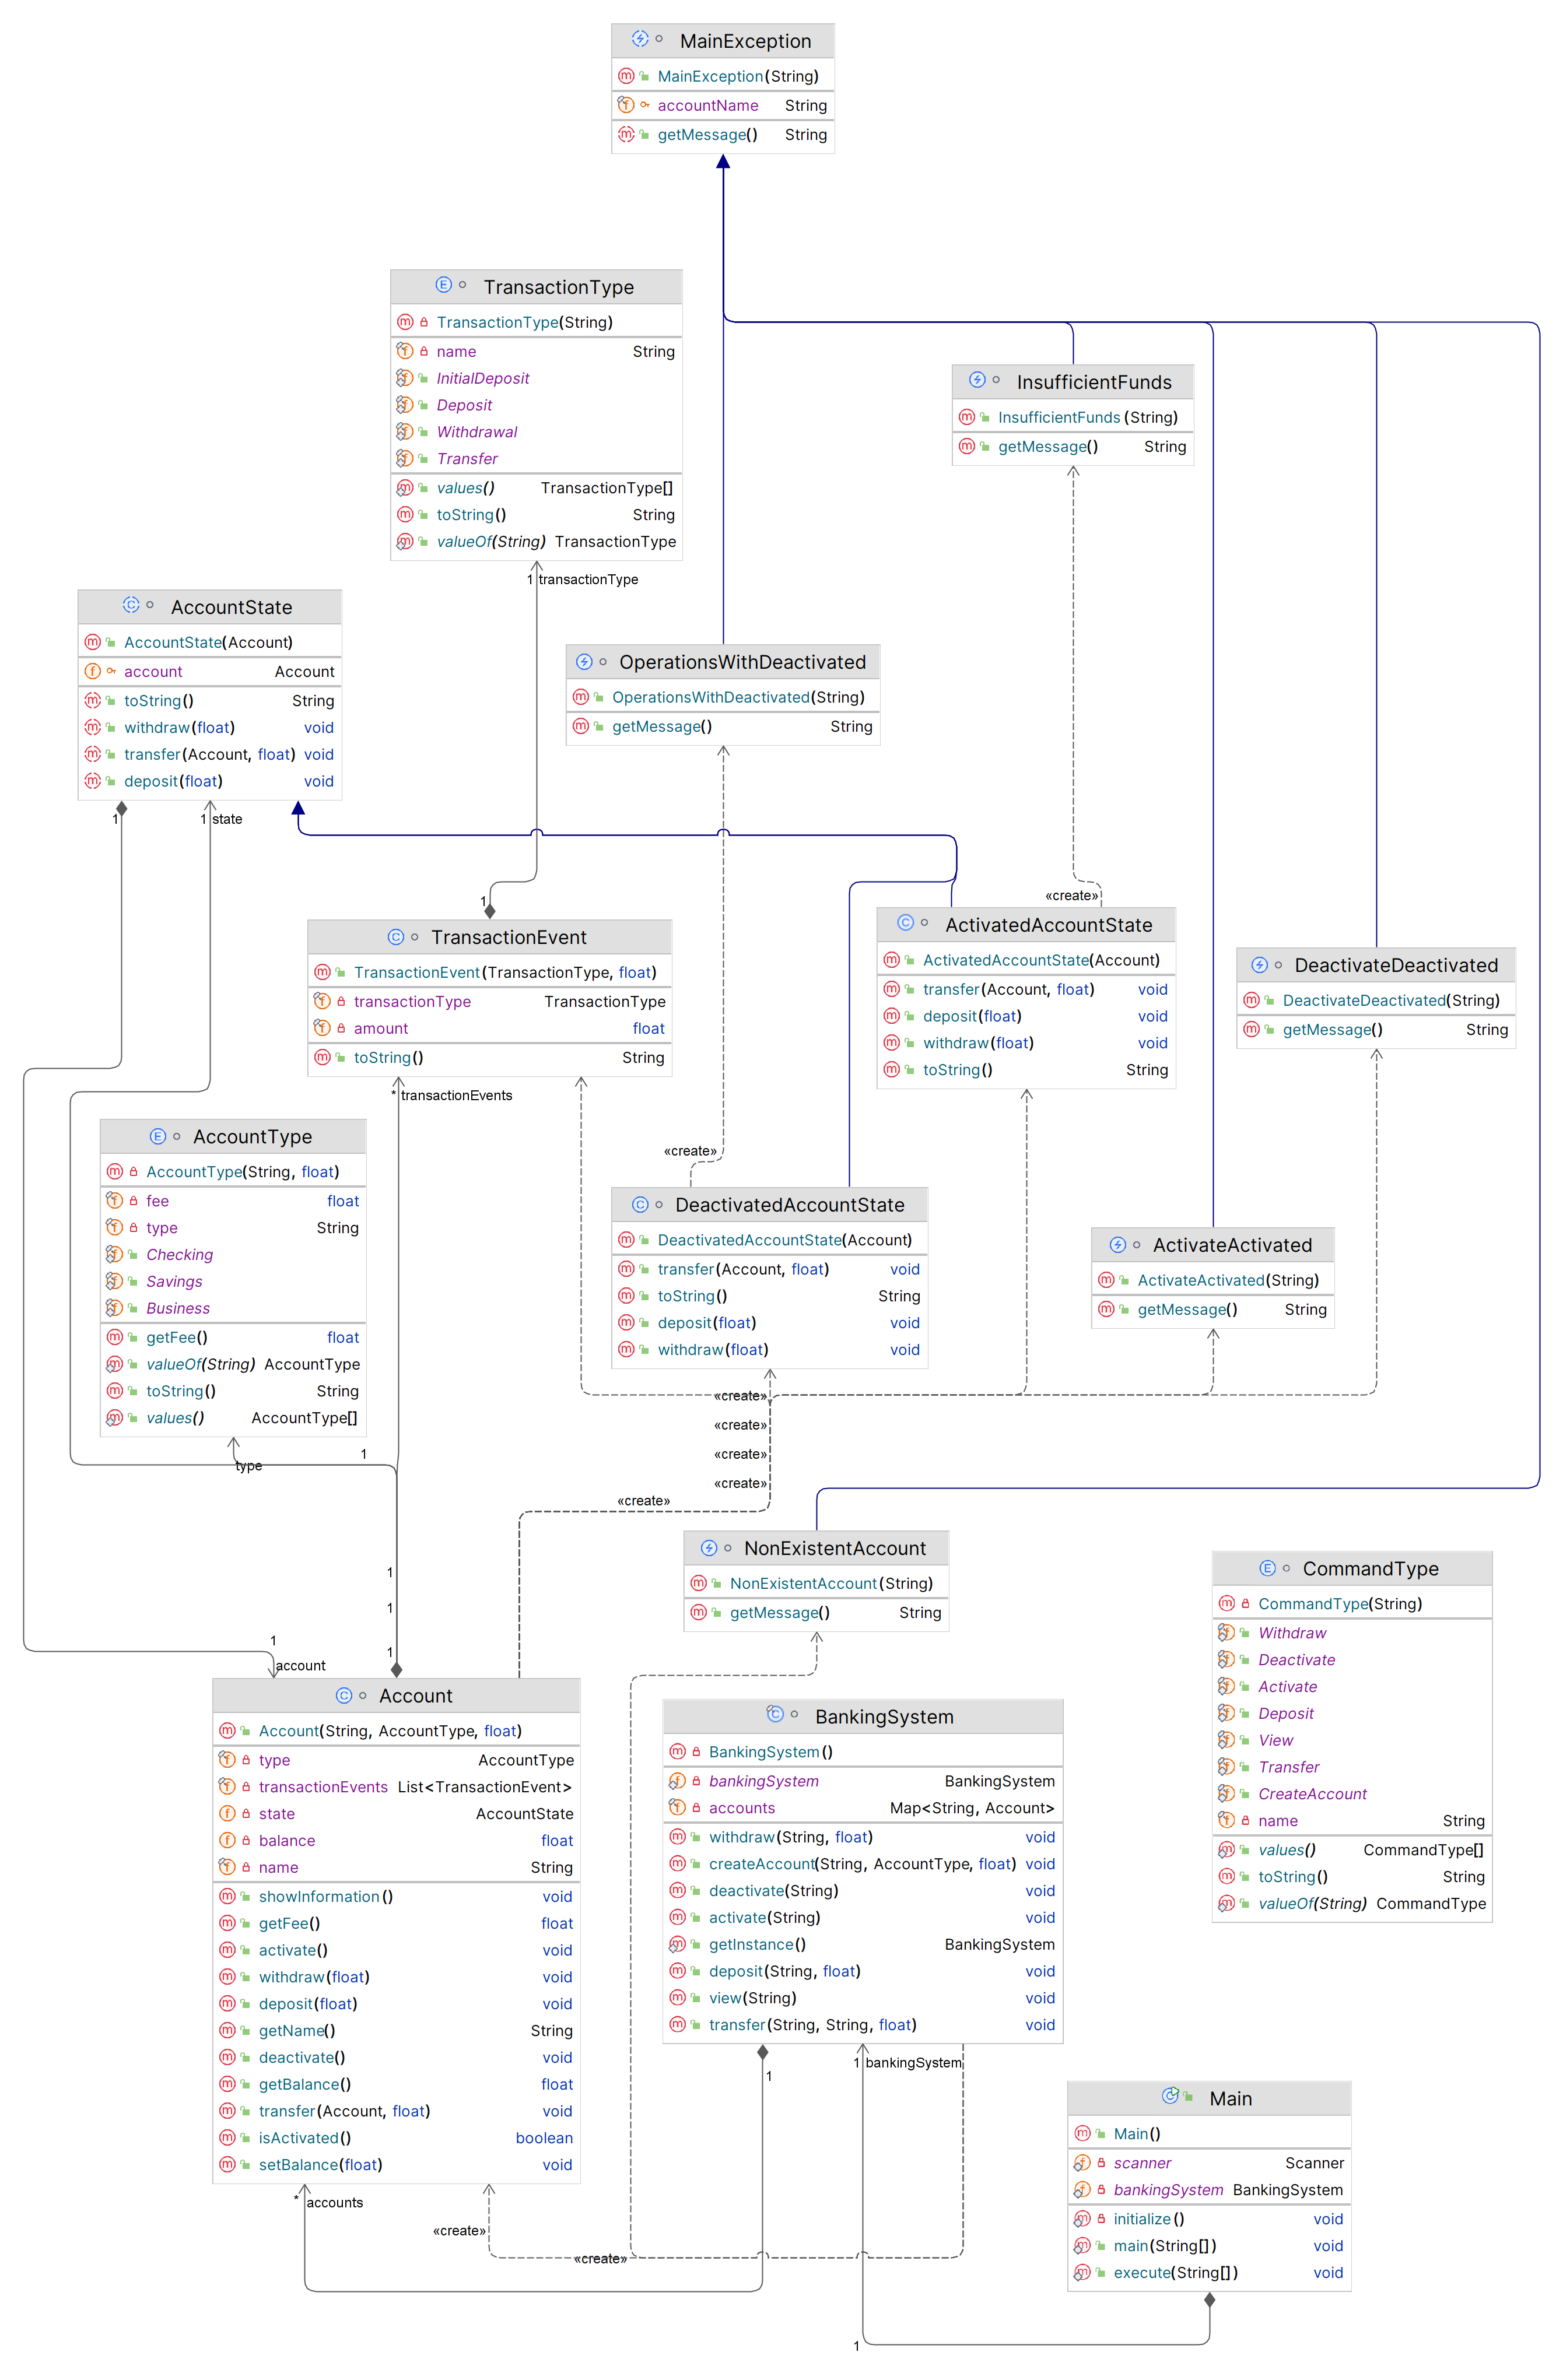
\includegraphics[width=\textwidth]{UML.png}
    \caption{UML diagram}
\end{figure}

\end{document}
